\documentclass[9pt]{article}

\usepackage{amsmath}
\usepackage{tcolorbox}
% `parskip` removes indentation for all paragraphs: http://tex.stackexchange.com/a/55016
\usepackage{parskip}
% Allows us to color rows / cols of a table.
% See https://texblog.org/2011/04/19/highlight-table-rowscolumns-with-color/
\usepackage{color, colortbl}

\usepackage{hyperref}
\graphicspath{{images/ps8a/}}

\leftmargin=0.25in
\oddsidemargin=0.25in
\textwidth=6.0in
\topmargin=-0.25in
\textheight=9.25in

\definecolor{Gray}{gray}{0.9}

\begin{document}

\begin{center}
  \large\textbf{MIT 18.01 Problem Set 8A Unofficial Solutions}
\end{center}

\begin{tcolorbox}
  \textbf{4E-2} Find the rectangular equation for $x = t + 1/t$ and $y = t - 1/t$ (compute $x^2$ and $y^2$).
\end{tcolorbox}

\begin{align*}
  x^2 &= t^2 + 2 + 1/t^2 \\
  y^2 &= t^2 - 2 + 1/t^2 \\
  y^2 &= x^2 -4 \\
  x^2 &- y^2 = 4
\end{align*}

This is an equation of a hyperbola centred at the origin with width 2.


\begin{tcolorbox}
  \textbf{4E-3} Find the rectangular equation for $x = 1 + sin\ t, y = 4 + cos\ t$
\end{tcolorbox}

\begin{align*}
  x^2 &= 1 + 2sin\ t + sin^2\ t \\
  y^2 &= 16 + 8sin\ t + cos^2\ t \\
  x^2 + y^2 &= 17 + 2sin\ t + 8cos\ t + sin^2\ t + cos^2\ t \\
  &= 18 + 2(sin\ t + 4cos\ t) \\
  &= 2(1 + sin\ t) + 8(4 + cos\ t) - 16 \\
  &= 2x + 8y - 16
\end{align*}

Then

\begin{align*}
  x^2 - 2x + y^2 - 8y + 16 &= 0 \\
  (x-1)^2 + (y-4)^2 - 1 &= 0 \\
  (x-1)^2 + (y-4)^2 &= 1
\end{align*}

This is an equation of a circle with radius 1 centred at $(1, 2)$.


\begin{tcolorbox}
  \textbf{4E-8} At noon, a snail starts at the center of an open clock face. It creeps at a steady rate along the hour hand, reaching the end of the hand at 1:00 PM. The hour hand is 1 meter long. Write parametric equations for the position of the snail at time t, in some reasonable xy-coordinate system.
\end{tcolorbox}

The average velocity of the snail is 1 metre / h. Let the centre of the clock be the origin.

Treat the positive x-axis as 0 radians. When the hour hand is 12pm, the angle with respect to the positive x-axis is $\pi / 2$ radians. When the hour hand is at 1pm, the angle with respect to the positive x-axis is $\pi / 3$ radians.

Hence, the angle traversed by the hour hand from 12pm to 1pm is $\pi / 6$ radians.

\begin{align*}
  x = t cos\ \theta = t\ cos(\frac{\pi}{2} - \frac{\pi}{6}t) \\
  y = t sin\ \theta = t\ sin(\frac{\pi}{2} - \frac{\pi}{6}t)
\end{align*}

\begin{center}
  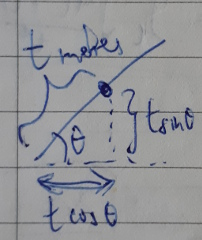
\includegraphics[scale=0.8]{p1_4e8.jpg}
\end{center}

Verification:

At $t = 0$ (12pm), the snail should be at $(0, 0)$.

\begin{align*}
  x &= 0\ cos(\frac{\pi}{2} - \frac{\pi}{6} \cdot 0) = 0 \\
  y &= 0\ sin(\frac{\pi}{2} - \frac{\pi}{6} \cdot 0) = 0
\end{align*}

At $t = 1$ (1pm), the snail should be at $(\frac{1}{2}, \frac{\sqrt{3}}{2})$ (draw out a right angle triangle with hypothenus 1 and the angle being $\pi / 3$ radians and you will see why these numbers):

\begin{align*}
  x &= 1\ cos(\frac{\pi}{2} - \frac{\pi}{6} \cdot 1) = cos(\frac{\pi}{3}) = \frac{1}{2} \\
  y &= 1\ sin(\frac{\pi}{2} - \frac{\pi}{6} \cdot 1) = sin(\frac{\pi}{3}) = \frac{\sqrt{3}}{2}
\end{align*}


\begin{tcolorbox}
  \textbf{4F-1d} Find the arclength of $y = (1/3)(2 + x^2)^{3/2},\ 1 \leq x \leq 2$.
\end{tcolorbox}

\begin{align*}
  \frac{dy}{dx} &= \frac{1}{2}(2x)(2 + x^2)^{1/2} = x(2 + x^2)^{1/2} \\
  \sqrt{1 + (\frac{dy}{dx})^2} &= \sqrt{1 + (x(2 + x^2)^{1/2})^2} \\
  &= \sqrt{1 + x^2(2 + x^2)} \\
  &= \sqrt{1 + 2x^2 + x^4} \\
  &= \sqrt{(x^2 + 1)^2} \\
  &= x^2 + 1 \\
\\
  ds &= x^2 + 1\ dx
\end{align*}

Arc length:

\begin{align*}
  \int_{1}^{2} x^2 + 1\ dx &= \frac{x^3}{3} + x \bigg]_{1}^{2} \\
  &= \frac{2^3}{3} + 2 - (\frac{1}{3} + 1) \\
  &= \frac{8}{3} + 2 - \frac{1}{3} - 1 \\
  &= \frac{10}{3}
\end{align*}


\begin{tcolorbox}
  \textbf{4F-4} Find the length of the curve $x = t^2$, $y = t^3$ for $0 \leq t \leq 2$.
\end{tcolorbox}

\begin{align*}
  \frac{dx}{dt} &= 2t \\
  \frac{dy}{dt} &= 3t^2 \\
  ds &= \sqrt{(\frac{dx}{dt})^2 + (\frac{dy}{dt})^2} \\
  &= \sqrt{(2t)^2 + (3t^2)^2} \\
  &= \sqrt{4t^2 + 9t^4} \\
  &= t\sqrt{4 + 9t^2} \\
  \int_{s_0}^{s_1} ds &= \int_{0}^{2} t\sqrt{4 + 9t^2} dt \\
  &= \frac{2/3 \cdot (4 + 9t^2)^{3/2}}{18} \bigg]_{0}^{2} \\
  &= \frac{1}{27} (4 + 9t^2)^{3/2} \bigg]_{0}^{2} \\
  &= \frac{1}{27} ((4 + 9(2)^2)^{3/2} - (4 + 9(0)^2)^{3/2}) \\
  &= \frac{1}{27} ((4 + 36)^{3/2} - 4^{3/2}) \\
  &= \frac{1}{27} (40^{3/2} - 8) \\
\end{align*}


\begin{tcolorbox}
  \textbf{4F-5} Find an integral for the length of the curve given parametrically in Exercise 4E-2 for $1 \leq t \leq 2$. Simplify the integrand as much as possible but do not evaluate.
\end{tcolorbox}

What is given in 4E-2: $x = t + 1 / t$, $y = t - 1 / t$.

\begin{align*}
  \frac{dx}{dt} &= 1 - \frac{1}{t^2} \\
  \frac{dy}{dt} &= 1 + \frac{1}{t^2} \\
  ds &= \sqrt{(\frac{dx}{dt})^2 + (\frac{dy}{dt})^2} dt \\
  &= \sqrt{(1 - \frac{1}{t^2})^2 + (1 + \frac{1}{t^2})^2} dt \\
  &= \sqrt{1 - \frac{2}{t^2} + \frac{1}{t^4} + 1 + \frac{2}{t^2} + \frac{1}{t^4}} dt \\
  &= \sqrt{2 + \frac{2}{t^4}} dt \\
  &= \sqrt{\frac{2t^4 + 2}{t^4}} dt \\
  \int_{s_0}^{s_1} ds &= \int_{1}^{2} \sqrt{\frac{2t^4 + 2}{t^4}} dt
\end{align*}


\begin{tcolorbox}
  \textbf{4F-8)} Find the length of the curve $x = e^t cos\ t$, $y = e^t sin\ t$ for $0 \leq t \leq 10$.
\end{tcolorbox}

\begin{align*}
  x^2 + y^2 &= e^{2t} cos^2\ t + e^{2t} sin^2\ t = e^{2t} \\
  \frac{dx}{dt} &= e^t cos\ t - e^t sin\ t \\
  \frac{dy}{dt} &= e^t sin\ t + e^t cos\ t \\
\end{align*}

\begin{align*}
  (\frac{dx}{dt})^2 + (\frac{dy}{dt})^2 &= e^{2t} cos^2\ t - 2e^{2t} cos\ t\ sin\ t + e^{2t}sin^2\ t + e^{2t}sin^2\ t + 2e^{2t}sin\ t\ cos\ t + e^{2t}cos^2\ t \\
  &= e^{2t} cos^2\ t + e^{2t}sin^2\ t + e^{2t}sin^2\ t + e^{2t}cos^2\ t \\
  &= 2 e^{2t}
\end{align*}

\begin{align*}
  ds &= \sqrt{(\frac{dx}{dt})^2 + (\frac{dy}{dt})^2}\ dt \\
  &= \sqrt{2e^{2t}}\ dt \\
  &= \sqrt{2}\ e^{t}\ dt \\
  \int_{s_0}^{s_1} ds &= \int_{0}^{10} \sqrt{2}\ e^t\ dt \\
  &= \sqrt{2}\ e^t\ \bigg]_{0}^{10} \\
  &= \sqrt{2}\ (e^{10} - e^{0}) \\
  &= \sqrt{2}\ (e^{10} - 1)
\end{align*}


\begin{tcolorbox}
  \textbf{4G-2} Find the area of the segment of $y = 1 - 2x$ in the first quadrant revolved around the x-axis.
\end{tcolorbox}

\begin{align*}
  ds &= \sqrt{1 + (\frac{dy}{dx})^2} \ dx \\
  &= \sqrt{1 + (-2)^2} \ dx \\
  &= \sqrt{5} \ dx
\end{align*}

Surface area:

\begin{align*}
  \int_{s_0}^{s_1} 2 \pi y \ ds &= \int_{0}^{1/2} 2 \pi (1 - 2x) \sqrt{5} dx \\
  &= 2 \sqrt{5} \pi \int_{0}^{1/2} 1 - 2x \ dx \\
  &= 2 \sqrt{5} \pi (x - x^2) \bigg]_{0}^{1/2} \\
  &= 2 \sqrt{5} \pi (\frac{1}{2} - \frac{1}{4})) \\
  &= \frac{\sqrt{5}}{2} \pi
\end{align*}


\begin{tcolorbox}
  \textbf{4G-5} Find the area of $y = x^2$, $0 \leq x \leq 4$ revolved around the y-axis.
\end{tcolorbox}

\begin{align*}
  ds &= \sqrt{1 + (\frac{dy}{dx})^2} \ dx \\
  &= \sqrt{1 + (\frac{1}{2}y^{-\frac{1}{2})^2}} \ dy \\
  &= \sqrt{1 + \frac{1}{4y}} \ dy
\end{align*}

Surface area:

\begin{align*}
  \int_{s_0}^{s_1} 2 \pi x \ ds &= \int_{0}^{16} 2 \pi x \sqrt{1 + \frac{1}{4y}} \ dy \\
  &= 2 \pi \int_{0}^{16} \sqrt{y} \sqrt{1 + \frac{1}{4y}} \ dy \\
  &= 2 \pi \int_{0}^{16} \sqrt{y + \frac{1}{4}} \ dy \\
  &= 2 \pi \frac{2}{3} (y + \frac{1}{4})^{3/2} \bigg]_{0}^{16} \\
  &= \frac{4 \pi}{3} (y + \frac{1}{4})^{3/2} \bigg]_{0}^{16} \\
  &= \frac{4 \pi}{3} ((\frac{65}{4})^{3/2} - \frac{1}{8})
\end{align*}


\begin{tcolorbox}
  \textbf{4H-1b} Give the polar coordinates for the rectangular coordinate $(-2, 0)$
\end{tcolorbox}

$r = 2$, $\theta = \pi$

Verify:

\begin{align*}
  x &= r\ cos \theta = 2 cos\ \pi = 2(-1) = 2 \\
  y &= r\ sin \theta = 2 sin\ \pi = 0
\end{align*}


\begin{tcolorbox}
  \textbf{4H-1f} Give the polar coordinates for the rectangular coordinate $(0, -2)$
\end{tcolorbox}

$r = 2$, $\theta = \frac{3\pi}{2}$

Verify:

\begin{align*}
  x &= r\ cos \theta = 2 cos\ \frac{3\pi}{2} = 0 \\
  y &= r\ sin \theta = 2 sin\ \frac{3\pi}{2} = 2(-1) = -2 \\
\end{align*}

Alternatively, $r = 2$, $\theta = -\frac{\pi}{2}$


\begin{tcolorbox}
  \textbf{4H-1g} Give the polar coordinates for the rectangular coordinate $(\sqrt{3}, -1)$
\end{tcolorbox}

$r = \sqrt{(\sqrt{3})^2 + (-1)^2} = \sqrt{3 + 1} = 2$

We know that $cos\ \theta = \frac{\sqrt{3}}{2}$ and $sin\ \theta = \frac{1}{2}$, so $\theta = \frac{\pi}{6}$

But in this case, we are in the 4th quadrant. So $\theta = 2 \pi - \frac{\pi}{6} = \frac{11 \pi}{6}$ or equivalently, $\theta = -\frac{\pi}{6}$.

Verify:

\begin{align*}
  x &= r\ cos \theta = 2 cos\ \frac{11\pi}{6} = 2 cos\ \frac{\pi}{6} = 2 \cdot \frac{\sqrt{3}}{2} = \sqrt{3} \\
  y &= r\ sin \theta = 2 sin\ \frac{11\pi}{6} = -2 sin\ \frac{\pi}{6} = -2 \cdot \frac{1}{2} = -1
\end{align*}


\begin{tcolorbox}
  \textbf{4H-2a} Find using two different methods the equation in polar coordinates for the circle of radius $a$ with center at $(a, 0)$ on the x-axis, as follows: \\
\\
  (i) write its equation in rectangular coordinates, and then change it to polar coordinates (substitute $x = r\ cos\ \theta$ and $y = r\ sin\ \theta$, and then simplify). \\
\\
  (ii) treat it as a locus problem: let $OQ$ be the diameter lying along the x-axis, and $P: (r, \theta)$ a point on the circle; use $\Delta OPQ$ and trigonometry to find the relation connecting $r$ and $\theta$.
\end{tcolorbox}

For part (i)

Equation of the circle is $(x - a)^2 + y^2 = a^2$.

Let $x = r\ cos\ \theta$, $y = r\ sin\ \theta$. Then

\begin{align*}
  (r\ cos\ \theta - a)^2 + (r\ sin\ \theta)^2 &= a^2 \\
  r^2\ cos^2\ \theta - 2ar\ cos\ \theta + a^2 + r^2\ sin^2\ \theta &= a^2 \\
  r^2 - 2ar\ cos\ \theta &= 0 \\
  r &= 2a\ cos\ \theta
\end{align*}

For part (ii)

\begin{center}
  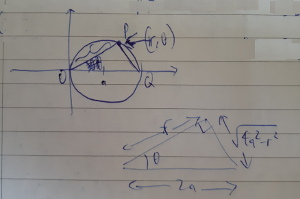
\includegraphics[scale=0.8]{p1_4h2.jpg}
\end{center}

\begin{align*}
  OQ &= 2a \\
  \angle OPQ &= \frac{\pi}{2} \\
  \angle POQ &= \theta \\
  \angle PQO &= \frac{\pi}{2} - \theta
\end{align*}

\begin{align*}
  cos\ \theta &= \frac{r}{2a} \\
  r &= 2a\ cos\ \theta
\end{align*}


\begin{tcolorbox}
  \textbf{4H-3f} For $r = a\ cos(2\theta)$ (4-leaf rose) \\
  (i) give the corresponding equation in rectangular coordinates; \\
  (ii) draw the graph; indicate the direction of increasing $\theta$
\end{tcolorbox}

For part (i)

\begin{align*}
  x = r\ cos\ \theta &= a\ cos(2 \theta)\ cos(\theta) \\
  y = r\ sin\ \theta &= a\ cos(2 \theta)\ sin(\theta) \\
\\
  x &= a\ cos(2 \theta)\ cos(\theta) \\
    &= a(cos^2 \theta - sin^2 \theta)\ cos\ \theta \\
    &= a(cos^3 \theta - cos\ \theta\ sin^2 \theta) \\
    &= a(cos^3 \theta - cos\ \theta\ (1 - cos^2 \theta)) \\
    &= a(cos^3 \theta - cos\ \theta\ + cos^3 \theta) \\
    &= a(2\ cos^3 \theta - cos\ \theta) \\
\\
  y &= a\ cos(2 \theta)\ sin(\theta) \\
  &= a\ (cos^2 \theta - sin^2 \theta)\ sin(\theta) \\
  &= a\ (1 - sin^2 \theta - sin^2 \theta)\ sin(\theta) \\
  &= a\ (1 - 2\ sin^2 \theta)\ sin(\theta) \\
  &= a\ (sin\ \theta - 2\ sin^3 \theta) \\
\\
  x^2 &= a^2 (2\ cos^3 \theta - cos\ \theta)^2 \\
  &= a^2(4\ cos^6 \theta - 4\ cos^4 \theta + cos^2 \theta) \\
\\
  y^2 &= a^2\ (sin\ \theta - 2\ sin^3 \theta)^2 \\
  &= a^2\ (4\ sin^6\ \theta - 4\ sin^4 \theta + sin^2 \theta) \\
\\
  r &= a\ cos(2\theta) = a(cos^2 \theta - sin^2 \theta) \\
  r^3 &= ar^2\ cos(2\theta) \\
  &= a(r^2 cos^2 \theta - r^2 sin^2 \theta) \\
  &= a(x^2 - y^2)
\end{align*}

Using polar coordinates, we know that $r = \sqrt{x^2 + y^2}$. Therefore $r^3 = (\sqrt{x^2 + y^2})^3$.

Equating $r^3 = a(x^2 - y^2)$ and $r^3 = (\sqrt{x^2 + y^2})^3$:

\begin{align*}
  a(x^2 - y^2) &= \sqrt{(x^2 + y^2)}^{3} \\
  (x^2 + y^2)^{3/2} &= a(x^2 - y^2)
\end{align*}

For part (ii)

\begin{center}
  \begin{tabular}{|c|c|}
    \hline
    \rowcolor{Gray}
    $\theta$ & $r = a\ cos(2 \theta)$ \\ \hline
    $0$ & $a\ cos(0) = a$ \\ \hline
    $\pi / 6$ & $a\ cos(\pi / 3) = a / 2$ \\ \hline
    $\pi / 4$ & $a\ cos(\pi / 2) = 0$ \\ \hline
    $\pi / 3$ & $a\ cos(2 \pi / 3) = -a / 3$ \\ \hline
    $\pi / 2$ & $a\ cos(\pi) = -a$ \\ \hline
    $2 \pi / 3$ & $a\ cos(4 \pi / 3) = -a / 2$ \\ \hline
    $3 \pi / 4$ & $a\ cos(3 \pi / 2) = 0$ \\ \hline
    $5 \pi / 6$ & $a\ cos(5 \pi / 3) = a / 2$ \\ \hline
    $\pi$ & $a\ cos(2 \pi) = a$ \\ \hline
    $7 \pi / 6$ & $a\ cos(7 \pi / 3) = a / 2$ \\ \hline
    $5 \pi / 4$ & $a\ cos(5 \pi / 2) = 0$ \\ \hline
    $3 \pi / 2$ & $a\ cos(3 \pi) = -a$ \\ \hline
    $5 \pi / 3$ & $a\ cos(10 \pi / 3) = -a / 2$ \\ \hline
    $7 \pi / 4$ & $a\ cos(7 \pi / 2) = 0$ \\ \hline
    $11 \pi / 6$ & $a\ cos(11 \pi / 3) = a / 2$ \\ \hline
    $2 \pi$ & $a\ cos(4 \pi) = a$ \\ \hline
  \end{tabular}
\end{center}

\begin{center}
  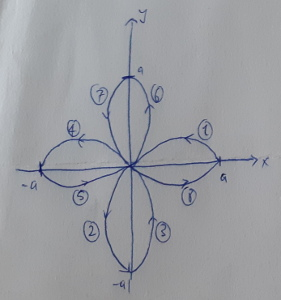
\includegraphics[scale=0.8]{p1_4h3.jpg}
\end{center}


\begin{tcolorbox}
  \textbf{4I-2} Find the area of one leaf of a three-leaf rose $r = a\ cos(3 \theta)$.
\end{tcolorbox}

\begin{center}
  \begin{tabular}{|c|c|}
    \hline
    \rowcolor{Gray}
    $\theta$ & $r = a\ cos(3 \theta)$ \\ \hline
    $0$ & $a\ cos(0) = a$ \\ \hline
    $\pi / 12$ & $a\ cos(\pi / 4) = \sqrt{2} \ a / 2$ \\ \hline
    $\pi / 6$ & $a\ cos(\pi / 2) = 0$ \\ \hline
    $\pi / 3$ & $a\ cos(\pi) = -a$ \\ \hline
    $\pi / 2$ & $a\ cos(3 \pi / 2) = 0$ \\ \hline
    $2 \pi / 3$ & $a\ cos(2 \pi) = a$ \\ \hline
    $3 \pi / 4$ & $a\ cos(9 \pi / 4) = \sqrt{2} \ a / 2$ \\ \hline
    $5 \pi / 6$ & $a\ cos(5 \pi / 2) = 0$ \\ \hline
    $11 \pi / 12$ & $a\ cos(11 \pi / 4) = -\sqrt{2} \ a / 2$ \\ \hline
    $\pi$ & $a\ cos(3 \pi) = -a$ \\ \hline
  \end{tabular}
\end{center}

\begin{center}
  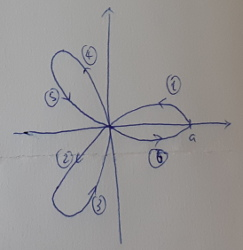
\includegraphics[scale=0.8]{p1_4i2.jpg}
\end{center}

Assume the petals are of equal area. We will find the area of the curve from $\theta = 0$ to $\theta = \pi / 6$ and multiply by 2.

\begin{center}
  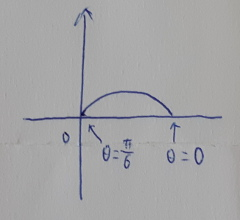
\includegraphics[scale=0.8]{p1_4i2-integration.jpg}
\end{center}

\begin{align*}
  2 \int_0^{\pi / 6} \frac{1}{2} r^2 d \theta &= \int_0^{\pi / 6} r^2 d \theta \\
  &= \int_0^{\pi / 6} a^2\ cos^2(3 \theta) d \theta \\
  &= a^2 \int_0^{\pi / 6} cos^2(3 \theta) d \theta \\
  &= a^2 \int_0^{\pi / 6} \frac{1 + cos(6 \theta)}{2} d \theta \\
  &= \frac{a^2}{2} \int_0^{\pi / 6} 1 + cos(6 \theta) d \theta \\
  &= \frac{a^2}{2} (\theta + \frac{sin(6 \theta)}{6}) \bigg]_0^{\pi / 6} \\
  &= \frac{a^2}{2} (\frac{\pi}{6} + \frac{sin(6 \cdot \pi / 6)}{6}) \\
  &= \frac{a^2}{2} (\frac{\pi}{6} + \frac{sin(\pi)}{6}) \\
  &= \frac{a^2 \pi}{12}
\end{align*}


\begin{tcolorbox}
  \textbf{4I-3} Find the area of the region $0 \leq r \leq e^{3 \theta}$ for $0 \leq \theta \leq \pi$
\end{tcolorbox}

Skipped.


\begin{tcolorbox}
  \textbf{Q1a)} Find the algebraic equation in $x$ and $y$ for the curve \\
  \\
  $x = a\ cos^k t, y = a \ sin^k t$ \\
  \\
  Draw the portion of the curve $0 \leq t \leq \pi / 2$ in the three cases $k = 1, k = 2, k = 3$.
\end{tcolorbox}

Raising both $x$ and $y$ to the power $2/k$, we get

$x^{2/k} = a^{2/k} \ cos^2 t$

$y^{2/k} = a^{2/k} \ sin^2 t$

Summing them, we get $x^{2/k} + y^{2/k} = a^{2/k} cos^2 t + a^{2/k} sin^2 t = a^{2/k}$

For $k = 1$, this is $x^2 + y^2 = a^2$

\begin{center}
  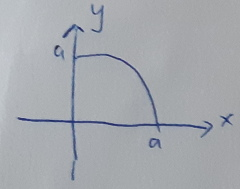
\includegraphics[scale=0.8]{1_keq1.jpg}
\end{center}

For $k = 2$, this is $x + y = a$ or equivalently, $y = a -x$.

Assuming $a > 0$, we get:

\begin{center}
  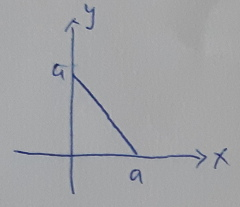
\includegraphics[scale=0.8]{1_keq2.jpg}
\end{center}

For $k = 3$, this is $x^{2/3} + y^{2/3} = a^{2/3}$

\begin{center}
  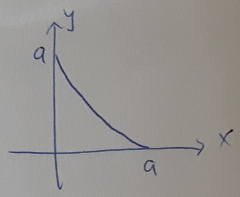
\includegraphics[scale=0.8]{1_keq3.jpg}
\end{center}


\begin{tcolorbox}
  Q1b) Without calculation, find the arclength in the cases $k = 1$ and $k = 2$.
\end{tcolorbox}

Frankly speaking, we need calculations for these.

Arc length for $k = 1$: $\frac{\pi a}{2}$

Arc length for $k = 2$: $\sqrt{2a^2}$


\begin{tcolorbox}
  Q1c) Find a definite integral formula for the length of the curve for general $k$. Then evaluate the integral in the three cases $k = 1, k = 2$ and $k = 3$. (Your answer in the first two cases should match what you found in part (b), but the calculation takes more time.)
\end{tcolorbox}

\begin{align*}
  x^{2/k} + y^{2/k} &= a^{2/k} \\
  y^{2/k} &= a^{2/k} - x^{2/k} \\
  y &= (a^{2/k} - x^{2/k})^{k/2} \\
  \frac{dy}{dx} &= \frac{k}{2}(a^{2/k} - x^{2/k})^{k/2 - 1}(-\frac{2}{k}x^{(2/k) - 1}) \\
\\
  ds &= \sqrt{1 + (dy/dx)^2} \ dx \\
  &= \sqrt{1 + (\frac{k}{2}(a^{2/k} - x^{2/k})^{k/2 - 1}(-\frac{2}{k}x^{(2/k) - 1}))^2} \ dx \\
  &= \sqrt{1 + (\frac{k^2}{4}(a^{2/k} - x^{2/k})^{k - 2} \ (\frac{4}{k^2}x^{2(2 - k)/k})} \ dx \\
  &= \sqrt{1 + (a^{2/k} - x^{2/k})^{k - 2} \ (x^{2(2 - k)/k})} \ dx \\
  \\
  \int_{s_0}^{s_1} ds &= \int_{0}^{a} \sqrt{1 + (a^{2/k} - x^{2/k})^{k - 2} \ (x^{2(2 - k)/k})} \ dx \\
\end{align*}

For $k = 1$

\begin{align*}
  \int_{0}^{a} \sqrt{1 + (a^2 - x^2)^{-1} \ x^2} \ dx &= \int_{0}^{a} \sqrt{1 + \frac{x^2}{a^2 - x^2}} \ dx \\
  &= \int_{0}^{a} \sqrt{\frac{a^2}{a^2 - x^2}} \ dx \\
  &= a \int_{0}^{a} \sqrt{\frac{1}{a^2 - x^2}} \ dx \\
\end{align*}

Let $x = a\ sin(u)$. Then $dx = a\ cos(u)\ du$. Substitute into above.

\begin{align*}
  a \int_{0}^{\pi / 2} \sqrt{\frac{1}{a^2 - a^2 sin^2(u)}} \ a \ cos(u) \ du &= a^2 \int_{0}^{\pi / 2} \sqrt{\frac{1}{a^2 cos^2(u)}} \ cos(u) \ du \\
  &= a^2 \int_{0}^{\pi / 2} \frac{cos(u)}{a\ cos(u)} \ du \\
  &= a \int_{0}^{\pi / 2} du \\
  &= a\ u \bigg]_0^{\pi / 2} \\
  &= a\pi / 2
\end{align*}

For $k = 2$

\begin{align*}
  \int_{0}^{a} \sqrt{1 + (a^{2/k} - x^{2/k})^{k - 2} \ (x^{2(2 - k)/k})} \ dx &= \int_0^a \sqrt{1 + (a - x)^0 \ x^{2(2 - 2) / 2}} \ dx \\
  &= \int_0^a \sqrt{1 + 1 \cdot \ x^0} \ dx \\
  &= \int_0^a \sqrt{2} \ dx \\
  &= \sqrt{2}\ x \bigg]_0^a \\
  &= \sqrt{2} \ a
\end{align*}

For $k = 3$

\begin{align*}
  \int_{0}^{a} \sqrt{1 + (a^{2/k} - x^{2/k})^{k - 2} \ (x^{2(2 - k)/k})} \ dx &= \int_{0}^{a} \sqrt{1 + (a^{2/3} - x^{2/3})^{3 - 2} \ (x^{2(2 - 3)/3})} \ dx \\
  &= \int_{0}^{a} \sqrt{1 + (a^{2/3} - x^{2/3}) \ (x^{-2/3})} \ dx \\
  &= \int_{0}^{a} \sqrt{1 + a^{2/3}x^{-2/3} - 1} \ dx \\
  &= \int_{0}^{a} \sqrt{a^{2/3}x^{-2/3}} \ dx \\
  &= \int_{0}^{a} a^{1/3}x^{-1/3} \ dx \\
  &= a^{1/3} \int_{0}^{a} x^{-1/3} \ dx \\
  &= a^{1/3} \cdot \frac{3}{2} x^{2/3} \bigg]_{0}^{a} \\
  &= a^{1/3} \cdot \frac{3}{2} a^{2/3} \\
  &= \frac{3}{2} a
\end{align*}


\begin{tcolorbox}
  Q2) The hyperbolic sine and cosine are defined by \\
  \\
  $cosh \ x = \frac{e^x + e^{-x}}{2}$, $sinh \ x = \frac{e^x - e^{-x}}{2}$ \\
  \\
  a) Show that \\
  \\
  i) $\frac{d}{dx}sinh \ x = cosh \ x$ and $\frac{d}{dx}cosh \ x = sinh \ x$. \\
  \\
  ii) $\frac{d}{dx}cosh^2 x = 1 + sinh^2 x$ \\
  \\
  iii) $cosh^2 x = \frac{1 + cosh \ 2x}{2}$.
\end{tcolorbox}

\begin{align*}
  \frac{d}{dx}sinh \ x &= \frac{d}{dx} \frac{e^x - e^{-x}}{2} \\
  &= \frac{e^x}{2} - (-1) \frac{e^{-x}}{2} \\
  &= \frac{e^x + e^{-x}}{2} \\
  &= cosh \ x
\end{align*}

\begin{align*}
  cosh^2 x &= (\frac{e^x + e^{-x}}{2})^2 \\
  &= \frac{e^2x + 2 + e^{-2x}}{4} \\
  sinh^2 x &= (\frac{e^x - e^{-x}}{2})^2 \\
  &= \frac{e^2x - 2 + e^{-2x}}{4} \\
  sinh^2 x + 1 &= \frac{e^2x - 2 + e^{-2x}}{4} + \frac{4}{4} \\
  &= \frac{e^2x + e^{-2x} + 2}{4} \\
  &= cosh^2 x
\end{align*}

\begin{align*}
  cosh\ 2x &= \frac{e^{2x} + e^{-2x}}{2} \\
  &= \frac{2e^{2x} + 2e^{-2x}}{4} \\
  &= \frac{2e^{2x} + 2e^{-2x} + 4 - 4}{4} \\
  &= \frac{2(e^{2x} + e^{-2x} + 2 - 2)}{4} \\
  &= \frac{2(e^{2x} + e^{-2x} + 2)}{4} - \frac{4}{4} \\
  &= 2cosh^2 x - 1 \\
  cosh^2 x &= \frac{cosh\ 2x + 1}{2}
\end{align*}


\begin{tcolorbox}
  Q2) The hyperbolic sine and cosine are defined by \\
  \\
  $cosh \ x = \frac{e^x + e^{-x}}{2}$, $sinh \ x = \frac{e^x - e^{-x}}{2}$ \\
  \\
  b) What curve is described parametrically by $x = cosh\ t$, $y = sinh\ t$? (Give the equation and its name.)
\end{tcolorbox}

Using $cosh^2 x = 1 + sinh^2 x$, $x = cosh\ x$ and $y = sinh \ t$, we have

$x^2 = 1 + y^2$

$x^2 - y^2 = 1$

This is a hyperbola.


\begin{tcolorbox}
  Q2) The hyperbolic sine and cosine are defined by \\
  \\
  $cosh \ x = \frac{e^x + e^{-x}}{2}$, $sinh \ x = \frac{e^x - e^{-x}}{2}$ \\
  \\
  c) The curve $y = cosh \ x$ is known as a \textit{catenary}. It is the curve formed by a chain whose two ends are held at the same height.\\
  i) Sketch the curve \\
  ii) Find its arclength from the lowest point to the point $(x_1, cosh\ x_1)$ for a fixed $x_1 > 0$
\end{tcolorbox}

$\frac{dy}{dx} cosh\ x = sinh\ x = \frac{e^x - e^{-x}}{2}$. This is $0$ when $e^x - e^{-x} = 0$, or $e^x = e^{-x}$, or $x = -x$, when $x = 0$.

When $x = 0$, $y = \frac{e^0 + e^{-0}}{2} = 1$. Hence $(0, 1)$ is a critical point.

$\frac{d^2 y}{dx^2} = cosh\ x = y$ . This is $0$ when $e^x + e^{-x} = 0$ which is impossible. There are no points of inflection.

Now we calculate the intercepts.

We know from above that when $x = 0$, $y = 1$. Because $e^x > 0$ and $e^{-x} > 0$, $y > 0$.

$\lim_{x \to -\infty} \frac{e^x + e^{-x}}{2} = \lim_{x \to -\infty} \frac{e^x}{2} + \lim_{x \to -\infty} \frac{e^{-x}}{2} = \infty$

Similarly, the limit as $x \to \infty$ is also $\infty$.

When $x = 0$, $\frac{d^2 y}{dx^2} = cosh \ x = \frac{e^x + e^{-x}}{2} = \frac{e^0 + e^{-0}}{2} = 1 > 0$ . Hence $(0, 1)$ is the minimum point.

\begin{center}
  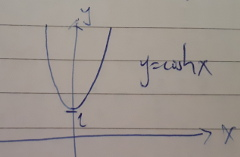
\includegraphics[scale=0.8]{2c.jpg}
\end{center}

\begin{align*}
  ds &= \sqrt{1 + (\frac{dy}{dx})^2} \ dx \\
  &= \sqrt{1 + sinh^2 \ x} \ dx \\
  &= \sqrt{cosh^2 x} \ dx \\
  &= cosh \ x \ dx
  \\
  \int_{s_0}^{s_1} ds &= \int_0^{x_1} cosh \ x \ dx \\
  &= sinh \ x \bigg]_0^{x_1} \\
  &= \frac{e^{x_1} + e^{-x_1}}{2} - \frac{e^0 - e^{-0}}{2} \\
  &= \frac{e^{x_1} + e^{-x_1}}{2} \\
  &= sinh \ x_1
\end{align*}


\begin{tcolorbox}
  Q2) The hyperbolic sine and cosine are defined by \\
  \\
  $cosh \ x = \frac{e^x + e^{-x}}{2}$, $sinh \ x = \frac{e^x - e^{-x}}{2}$ \\
  \\
  d) FInd the area of the surface of revolution formed by revolving the portion of the curve from part (c) around the $x$-axis This surface is known as a catenoid. It is interesting because it is the surface of least area connecting the two circles that form its edges. If you dip two circles of wire in a soap solution, then (with some caoxing) a soap film will form in this shape. In general, the soap films try to span a frame of wires with a surface with the least area possible.
\end{tcolorbox}

Surface area:

\begin{align*}
  \int_0^{x_1} 2 \pi y \ dx &= 2 \pi \int_0^{x_1} y \ dx \\
  &= 2 \pi \int_0^{x_1} cosh \ x \ dx \\
  &= 2 \pi sinh \ x \bigg]_0^{x_1} \\
  &= 2 \pi (\frac{e^{x_1} - e^{-x_1}}{2} - \frac{e^0 - e^{-0}}{2}) \\
  &= 2 \pi sinh \ x_1
\end{align*}

which is $2\pi$ times the arc length.


\begin{tcolorbox}
  Q3a) Find the area of the right triangle with vertices at $(x, y) = (0, 0)$, $(x, y) = (a, 0)$ and at $(x, y) = (a, h)$, using polar coordinates. (One of the less convenient ways to find the area of a triangle.)
\end{tcolorbox}

\begin{center}
  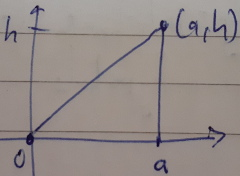
\includegraphics[scale=0.8]{3a.jpg}
\end{center}

Suppose $a > 0$, $h > 0$.

$r = \sqrt{a^2 + h^2}$

$\theta = tan^{-1} \frac{h}{a}$.

$tan \theta = \frac{h}{a}$.

\begin{align*}
  \int_{0}^{tan^{-1}(h/a)} \frac{1}{2} r^2 d \theta &= \frac{1}{2} \int_{0}^{tan^{-1}(h/a)} r^2 \ d \theta \\
  &= \frac{1}{2} \int_{0}^{tan^{-1}(h/a)} a^2 + h^2 \ d \theta \\
  &= \frac{a^2}{2} \int_{0}^{tan^{-1}(h/a)} 1 + \frac{h^2}{a^2} \ d \theta \\
  &= \frac{a^2}{2} \int_{0}^{tan^{-1}(h/a)} 1 + (tan \ \theta)^2 \ d \theta \\
  &= \frac{a^2}{2} \int_{0}^{tan^{-1}(h/a)} sec^2 \ \theta \ d \theta \\
  &= \frac{a^2}{2} tan \ \theta \bigg]_{0}^{tan^{-1}(h/a)} \\
  &= \frac{a^2}{2} [tan(tan^{-1}(h/a)) - tan(0)] \\
  &= \frac{a^2}{2} [\frac{h}{a} - 0] \\
  &= \frac{ah}{2}
\end{align*}


\begin{tcolorbox}
  Q3b) Find the equation in $(x, y)$ coordinates for the curve $r = 1 / (1 + sin\ \theta)$ and sketch it.
\end{tcolorbox}

\begin{align*}
  r &= \frac{1}{1 + sin\ \theta} \\
  r &+ r\ sin\ \theta = 1 \\
  r &+ y = 1 \\
  x &= r\ cos\ \theta = \frac{cos\ \theta}{1 + sin\ \theta} \\
  y &= r\ sin\ \theta = \frac{sin\ \theta}{1 + sin\ \theta} \\
  x^2 + y^2 &= \frac{cos^2 \theta + sin^2 \theta}{(1 + sin\ \theta)^2} = \frac{1}{(1 + sin\ \theta)^2} = r^2 \\
  r &= (x^2 + y^2)^{1/2} \\
  r + y &= (x^2 + y^2)^{1/2} + y = 1
\end{align*}

Hence the equation is $(x^2 + y^2)^{1/2} + y = 1$.

Skipping the sketch.


\begin{tcolorbox}
  Q3c) Find the area of the region $0 \leq r \leq 1 / (1 + sin\ \theta)$, $0 \leq \theta \leq \pi$, using the \textit{rectangular} coordinate formula you found in part (b).
\end{tcolorbox}

\begin{align*}
  (x^2 + y^2)^{1/2} + y &= 1 \\
  (x^2 + y^2)^{1/2} &= 1 - y \\
  x^2 + y^2 &= (1 - y)^2 \\
  x^2 = (1 - y)^2 - y^2 &= 1 - 2y \\
  y &= \frac{1 - x^2}{2}
\end{align*}

Area:

\begin{align*}
  \int_{-1}^1 \frac{1 - x^2}{2} dx &= (\frac{x}{2} - \frac{x^3}{6}) \bigg]_{-1}^1 \\
  &= \frac{1}{2} - \frac{1}{6} - (\frac{-1}{2} - \frac{(-1)^3}{6}) \\
  &= \frac{1}{2} - \frac{1}{6} + \frac{1}{2} - \frac{1}{6} \\
  &= \frac{2}{3}
\end{align*}


\begin{tcolorbox}
  Q3d) Find the area of the region in part (c) using polar coordinates. One way to evaluate the integral is to change variables to $u = \theta - \pi / 2$, and then use the half angle formula \\
  \\
  $1 + cos\ u = 2 cos^2(u/2)$ \\
  \\
  This area was already computed in part (c), but the polar coordinate formula is still valuable because it gives the area of any sector, not just the one that is bounded by a horizontal line. The area swept out from the viewpoint of the focus of an ellipse, parabola, or hyperbola is related by Kepler's law to the speed of planets and comets.
\end{tcolorbox}

Area:

\begin{align*}
  \int_0^{\pi} \frac{1}{2} r^2 d\theta = \frac{1}{2} \int_0^{\pi} (\frac{1}{1 + sin\ \theta})^2 d\theta
\end{align*}

Let $u = \theta - \pi / 2$. Then $du = d \theta$

When $\theta = 0$, $u = -\pi / 2$. When $\theta = \pi$, $u = \pi / 2$.

Then $sin\ \theta = sin(u + \pi / 2) = cos\ u$

\begin{align*}
  \frac{1}{2} \int_0^{\pi} (\frac{1}{1 + sin\ \theta})^2 d\ \theta &= \frac{1}{2} \int_{-\pi / 2}^{\pi / 2} (\frac{1}{2cos^2(u / 2)})^2\ du \\
  &= \frac{1}{2} \int_{-\pi / 2}^{\pi / 2} \frac{1}{4} sec^4(u / 2)\ du \\
\end{align*}

Let $w = tan(u / 2)$. Then $dw = \frac{1}{2} sec^2(u / 2) \ du$

\begin{align*}
  \int_{-\pi / 2}^{\pi / 2} sec^4(u / 2)\ du &= \int_{tan(-\pi / 2 / 2)}^{tan(\pi / 2 / 2)} sec^2(u / 2) \cdot sec^2(u / 2) \ du \\
  &= \int_{-1}^{1} (1 + tan^2(u / 2)) \cdot (2 \cdot \frac{1}{2} sec^2(u / 2)) \ du \\
  &= \int_{-1}^{1} (1 + w^2) \cdot 2 \ dw \\
  &= 2 \int_{-1}^{1} 1 + w^2 dw \\
  &= 2 (w + \frac{w^3}{3}) \bigg]_{-1}^1 \\
  &= 2 (1 + \frac{1}{3} - (-1 + \frac{(-1)^3}{3})) \\
  &= 2 (1 + \frac{1}{3} + 1 + \frac{1}{3}) \\
  &= 2 (2 + \frac{2}{3}) \\
  &= \frac{16}{3} \\
  \\
  \frac{1}{2} \int_{-\pi / 2}^{\pi / 2} \frac{1}{4} sec^4(u / 2)\ du &= \frac{1}{8} \int_{-\pi / 2}^{\pi / 2} sec^4(u / 2)\ du \\
  &= \frac{1}{8} \cdot \frac{16}{3} \\
  &= \frac{2}{3}
\end{align*}

\end{document}
